\documentclass[11pt, a4paper, ngerman]{arbeitsblatt}

\ladeModule{theme,qrcodes}

\ladeFach[]{informatik}

\aboptionen{
	name		= {J. Neugebauer},
	kuerzel 	= {Ngb},
	titel 		= {QR-Codes},
	reihe 		= {Informationen, Daten und Codierung},
	fach 		= {Informatik},
	kurs 		= {EF},
	nummer 		= {I.5},
	lizenz 		= {cc-by-nc-sa-4},
	version 	= {2021-09-14},
}

\begin{document}
\ReiheTitel

QR-Codes sind ein fester Bestandteil des täglichen Lebens. Man findet sie in
Zeitschriften, auf Plakaten und Visitenkarten, an Messeständen und
Museumsexponaten. QR-Codes sind die bekanntesten und im Alltag am häufigsten
verwendeten zweidimensionalen Codes. Die 2-D-Codes wurden ursprünglich zur
Kennzeichnung von Bauteilen in der Industrie und Raumfahrt entwickelt. Heute
ermöglichen sie unter anderem das Versenden von Briefen, das Bahnfahren und
geben mit wenigen Knopfdrücken den Zugang zu verschiedenen digitalen Medien
frei.

Der Begriff stammt aus dem Englischen und ist eine Abkürzung für Quick
Response, d. h. »schnelle Antwort«. Der erste QR-Code wurde im Jahr 1994 von
der Firma DENSO WAVE erfunden, einer Tochterfirma des japanischen
Automobilzulieferers DENSO Corporation, die für automatische Identifikation und
Datenerfassung (Auto-ID), Industrieroboter sowie Spezialelektronik für die
Automation in der Fertigung zuständig ist.

QR-Codes sind eine Codierung von binären Datenpaketen, die mit einer variablen
Fehlerkorrektur versehen sind, wodurch selbst teilweise verdeckte QR-Codes
erkannt werden können.

\begin{links}[.89]
\begin{aufgabe}
	Schau das Video unter \url{https://link.ngb.schule/video-qrcodes} (QR-Code
	rechts) und benenne dabei die freien Felder im Schema eines QR-Codes unten.
\end{aufgabe}
\end{links}\begin{rechts}[.09]
	\qrcode{https://link.ngb.schule/video-qrcodes}
\end{rechts}

\def\squaresize{.33}
\begin{center}
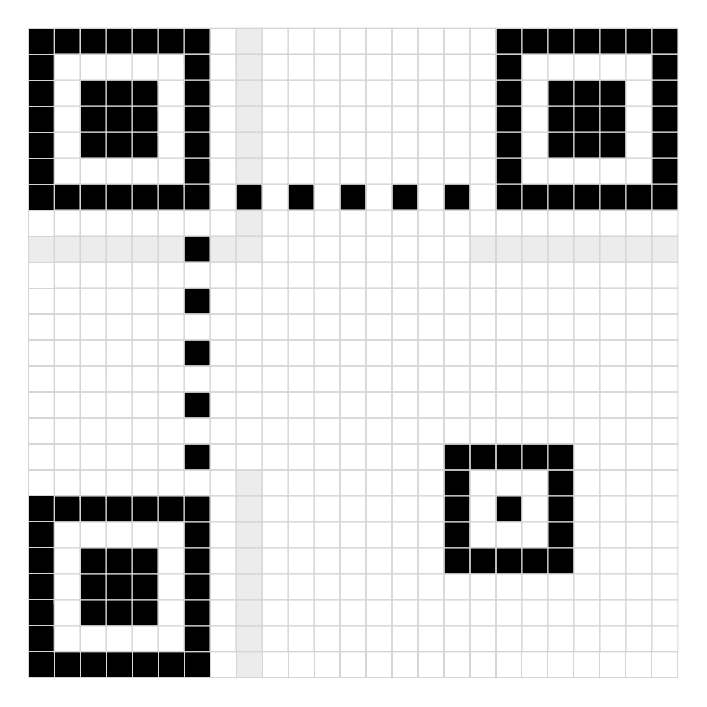
\begin{tikzpicture}[scale=.33]
	\foreach \i in {0,...,6} {
		\fill[black] (\i,0) |- +(1,1) |- cycle;
		\fill[black] (0,\i) |- +(1,1) |- cycle;
		\fill[black] (\i,6) |- +(1,1) |- cycle;
		\fill[black] (6,\i) |- +(1,1) |- cycle;

		\fill[black] (\i,24) |- +(1,1) |- cycle;
		\fill[black] (0,18+\i) |- +(1,1) |- cycle;
		\fill[black] (\i,18) |- +(1,1) |- cycle;
		\fill[black] (6,18+\i) |- +(1,1) |- cycle;

		\fill[black] (18+\i,24) |- +(1,1) |- cycle;
		\fill[black] (18,18+\i) |- +(1,1) |- cycle;
		\fill[black] (18+\i,18) |- +(1,1) |- cycle;
		\fill[black] (24,18+\i) |- +(1,1) |- cycle;
	}
	\foreach \i in {0,1,2} {
		\foreach \j in {0,1,2} {
			\fill[black] (2+\i,2+\j) |- +(1,1) |- cycle;
			\fill[black] (2+\i,20+\j) |- +(1,1) |- cycle;
			\fill[black] (20+\i,20+\j) |- +(1,1) |- cycle;
		}
	}
	\foreach \i in {0,...,4} {
		\fill[black] (20-\i,4) |- +(1,1) |- cycle;
		\fill[black] (16,4+\i) |- +(1,1) |- cycle;
		\fill[black] (20-\i,8) |- +(1,1) |- cycle;
		\fill[black] (20,4+\i) |- +(1,1) |- cycle;
	}
	\fill[black] (18,6) |- +(1,1) |- cycle;
	\foreach \i in {0,...,8} {
		\fill[gray!15!white] (\i,16) |- +(1,1) |- cycle;
		\fill[gray!15!white] (8,24-\i) |- +(1,1) |- cycle;
	}
	\foreach \i in {0,...,7} {
		\fill[gray!15!white] (17+\i,16) |- +(1,1) |- cycle;
		\fill[gray!15!white] (8,7-\i) |- +(1,1) |- cycle;
	}
	\foreach \i in {0,...,12} {
		\fill[black] (2*\i,18) |- +(1,1) |- cycle;
		\fill[black] (6,2*\i) |- +(1,1) |- cycle;
	}
	\foreach \i in {0,...,24} {
		\foreach \j in {0,...,24} {
			\draw[thin,gray!33!white] (\i,\j) |- +(1,1) |- cycle;
		}
	}
\end{tikzpicture}
\end{center}

\end{document}
